\chapter{Proof of correctness for chapter \ref{chapter:conformingsubdivision}}\label{appendix:proofs}

The following section includes all the proofs for correctness of the discussed topics in the chapter. These are taken from \cite{HershbergerS99}, and included for completeness.

\section{Correctness for \textbf{build-subdivision}}

\begin{Lemma} (Lemma 6.2 in \cite{HershbergerS99}) \\
The subdivision computed by the algorithm \textbf{build-subdivision} satisfies Invariants 1 and 2.
\end{Lemma}

\begin{proof}
We prove by induction that the invariants hold inside the family of quads $\mathcal{Q}(i)$, for all $i$. The initial family of quads $\mathcal{Q}(-2)$ clearly satisfies the two invariants. We show that no step of the algorithm \textbf{build-subdivision} ever violates these invariants. Step $2-8$ compute $\mathbf{growth}(S)$ for each equivalence class of $\mathcal{Q}(i)$, and then computes $\mathcal{Q}$. No new edges are drawn in this step.\\

The only edges drawn in step $9-12$ are on the boundaries of simple components. Let $q$ be $(i-2)$-quad that is a simple component of $\mathcal{Q}(i-2)$. By definition, the single $(i-4)$-quad of $\mathcal{Q}(i-4)$ contained in $q$ lies in its core, and thus is separated from the outer boundary of $q$ by a gap of at least $2^{i-2}$ on all sides. Hence the edge already drawn in the core satisfy Invariant 1: they have length no more than $2^{i-2}$ (actually $2^{i-4}$, except when $i=0$), and are separated from the boundary of $q$ by a gap of at least $2^{i-2}$. We draw the boundary of $q$ in step $9-12$; since any previously drawn edges within $q$ withing $q$ lie in its core, the new edges satisfy Invariant 1. Invariant 2 holds vacuously. \\

Steps $13-19$ subdivides the region covered by each complex component $S$. Again, the boundary of $S$ is separated from any components of $\mathcal{Q}(i-2)$ contained in it by a gap at least the width of an $i$-box. Step $18$ add $(i-2)$-boxes to pad the region covered by $\mathcal{Q}(i-2)$ out to the boundaries of $i$-boxes. By Invariant 2, the newly drawn boxes satisfy Invariant 1 with respect to the previously drawn edges; they clearly satisfy Invariant 1 with respect to each other's edges. Step $19$ pacts the area between the core and the boundary of $S$ with $i$-boxes, and breaks the segments incident to previously drawn cells into four pieces to guarantee Invariant 1 with respect to those cells. (The previously drawn edges on the core boundary have length $2^{i-2}$, so by induction the cells incident to them have side lengths at least $2^{i-2}$. It follows that the cells inside the core satisfy Invariant 1 with respect to the newly drawn segments of length $2^{i-2}$.) The segments of the boundary of $S$ are unbroken, so Invariant 2 holds at the next stage of the algorithm. This completes the proof.
\end{proof}

\begin{Lemma}(Lemma 6.3 from \cite{HershbergerS99}) \label{lemma:6.3HershbergerS99}\\
The subdivision produced by \textbf{build-subdivision} has size $O(n)$.
\end{Lemma}

\begin{proof}
We show that the algorithm draws a linear number of edges altogether. The number of edges drawn in step $9-12$ is proportional to the number drawn in $13-19$, so we draw a constant number of edges in step $9-12$ for each simple component that merges to form a complex component at the next stage. The number of edges drawn in step $13-19$ for a complex component $S$ if $O(|S'|)$, the number of $(i-2)$-quads whose growths constitute $S$. The key observation in proving the linear bound is that the total size of $\mathcal{Q}$ decreases every two stages by an amount proportional to the total number of quads in complex components. This fact, which we prove in Lemma \ref{lemma:growthgrowthS}, can be expressed as follows: If $e_i$ edges are drawn in stage $i$, then
$$|\mathcal{Q}(i+2)| \leq |\mathcal{Q}(i-2)| - \Theta(e_i)$$
That is, there exists an absolute constant $\beta$ such that
$$\beta\cdot e_i \leq |\mathcal{Q}(i-2)|-|\mathcal{Q}(i+2)|$$
If we sum this inequality over all even $i \geq 0$, the right hand side telescopes, and we obtain 
$$\beta \cdot \sum_i e_i \leq |\mathcal{Q}(-2)| + |\mathcal{Q}(0)| - 2$$
Since $|\mathcal{Q}(-2)|=n$, we have $\sum_i e_i \leq (2n-2)/\beta$. The number of edges in the subdivision is $O(n)$.
\end{proof}

\begin{Lemma} (Lemma 6.4 in \cite{HershbergerS99}) \label{lemma:6.4HershbergerS99}\\ 
The subdivision produced by \textbf{build-subdivision} is strongly 1-conforming and satisfies the following additional properties:
\begin{enumerate}
	\item all edges of the subdivision are horizontal or vertical
    \item each face is either a square or a square-annulus (with subdivided boundary)
    \item each annulus has the minimum clearance property
    \item each face has the uniform edge property, and
    \item every point of $V$ is contained in a square face.
\end{enumerate}
\end{Lemma}

\begin{proof}
Strong 1-conformity is a consequence of Invariant 1, as we now show. Condition C1. from definition \ref{def:wellcoveringwithpara} is trivially true, since each point is initially enclosed by a square. 

To establish well-covering, condition C2., let $I(e)$ be the union of the (at most 6) cells incident to an edge $e$. By Invariant 1, the distance from $e$ to any edge outside or on the boundary of $I(e)$ is at least $|e|$. Edge $e$ may be collinear with other edges of the two cells on whose boundary it lies. We define $\mathcal{C}(e)$ to be the set of cells incident to any of these collinear edges; $\mathcal{U}(e)$, the union of these cells, is a superset of $I(e)$. See Figure \ref{fig:wellcoveringregiondashed}. Because the two cells with $e$ as a boundary edge meet only along edges collinear with $e$, this definition of $\mathcal{U}(e)$ means that for any edge $f$ on or outside the boundary of $\mathcal{U}(e)$, if $I(f)$ does not contain both cells incident to $e$. But this implies, by Invariant 1, that $e$ is on or outside the boundary of $I(f)$, and hence the distance from $e$ to $f$ is at least $|f|$. Edge $e$ certainly lies in the interior of $\mathcal{U}(e)$ (condition W1. from definition \ref{def:aconformingsubdivision}). \\

Condition W2. follows because $\mathcal{C}(e)$ is the union of $I(e')$ for $O(1)$ edges $e'$ collinear with $e$, $|I(e')|\leq 6$ for each $e'$, and each cell has constant complexity. As noted above, the minimum distance between $e$ and any edge $f$ on or outside the boundary of $\mathcal{U}(e)$ is at least $\max(|e|,|f|)$, which establishes condition W3'. \\

Condition C3. follows from the observation that a well-covering region $\mathcal{U}(e)$ includes a vertex $v$ of $V$ if and only if $e$ is an edge of the square containing $v$. This is because each vertex-containing square is the inner square of a square annulus in the subdivision. No edge belongs to two such squares, so condition C3 holds. \\

Properties (1)-(5) holds by construction. this completes the proof.
\end{proof}

\textbf{Conforming Subdivision Theorem:} \\
	For any $\alpha\geq 1$, every set of $n$ points in the plane admits a strong
	$\alpha$-conforming subdivision of $O(\alpha n)$ size satisfying the
	following additional properties:
\begin{enumerate}	
	\item All edges of the subdivision are horizontal or vertical,
	\item Each face is either a square of a square-annulus, with subdivided
		boundary,
	\item Each annulus has the minimum clearance property,
	\item Each face has the uniform edge property, and
	\item Every data point is contained in the interior of a square face
\end{enumerate}
	Such a subdivision can be computed in time $O(\alpha n + n\log n)$.

\begin{proof}
Lemma \ref{lemma:6.1HershbergerS99}, \ref{lemma:6.3HershbergerS99}, \ref{lemma:6.4HershbergerS99} and \ref{lemma:6.11HershbergerS99} establish the theorem.
\end{proof}

\section{Correctness for \textbf{growth}} \label{section:correctnessgrowth}

\begin{Lemma} (Lemma 6.5 in \cite{HershbergerS99}) \label{lemma:growthgrowthS}\\
Let $S \subset \mathcal{Q}(i)$ be a set of two or more $i$-quads such that $\mathbf{growth}(S)$ is a complex component under the equivalence relation $\equiv_{i+2}$. Then $|\mathbf{growth}(\mathbf{growth}(S))| \leq \kappa|S|$, for an absolute constant $0 < \kappa < 1$.
\end{Lemma}

\begin{proof}
We show that either $|\mathbf{growth}(S)| < (3/4)|S|$, or at least half of the quads of $\mathbf{growth}(S)$ can be contained in a $2 \times 2$ array of $(i+2)$-boxes with some other quad of $\mathbf{growth}(S)$. 

If $|\mathbf{growth}(S)| < (3/4)|S|$, then we are done, because the following inequality obviously holds: $|\mathbf{growth}(\mathbf{growth}(S))| \leq |\mathbf{growth}(S)| \leq (3/4)|S|$. Therefore, suppose that $|\mathbf{growth}(S)| \geq (3/4)|S|$. Then at least half the $i$-quads of $S$ are not matched in step 5 of the function $\mathbf{growth}(S)$, and their growths contribute more than half of the $(i+2)$-quads of $\mathbf{growth}(S)$. Consider on such $i$-quad $q\in S$. Since $S$ is nonsingleton equivalence class, there exists another $i$-quad $q'\in S$ that overlaps $q$ Let $\bar{q}=\mathbf{growth}(q)$ and $\bar{q}' = \mathbf{growth}(q')$. By assumption $\bar{q} \neq \bar{q}'$. The cores of $\bar{q}$ and $\bar{q}'$ both contain the overlap region $q\cap q'$, so the cores must overlap. Therefore both cores are contained within a $3 \times 3$ array of $(i+2)$-boxes, and both the $(i+2)$-quads $\bar{q}$ and $\bar{q}'$ are contained within a $5 \times 5$ array of $(i+2)$-boxes. This ensures that $\bar{q}$ and $\bar{q}'$ are joined by an edge in the graph of $\mathbf{growth}(S)$: any two $(i+2)$-quads whose bounding box is contained in a $5 \times 5$ array of $(i+2)$-boxes can be covered by an $2 \times 2$ array of $(i+4)$-boxes. Hence the number of edges in the maximal matching of $\mathbf{growth}(S)$ is $\Omega(|S|)$, which proves the inequality $|\mathbf{growth}(\mathbf{growth}(S))| \leq \kappa|S|$ for some $\kappa < 1$.
\end{proof}

\section{Proofs for correctness of the conforming subdivision}

The following lemma proves that one can modify a strong conforming subdivision of 
obstacle vertices to obtain a conforming subdivision of the free space. This 
subdivision of free space has the additional property that each obstacle vertex is 
incident to a transparent edge. It should be noted that the shortest path algorithm of 
\cite{HershbergerS99} computes the distance from the source of the endpoints of all 
the transparent edges. The condition that each obstacle vertex is incident to a 
transparent edge ensures the distance to each obstacle vertex is correctly computed.

\begin{Lemma}(Lemma 2.2 in \cite{HershbergerS99})
\label{lemma:admitsa2conformingsubdivision}\\
Every family of disjoint simple polygons with a total of n vertices admits a 2-conforming
subdivision of the free space with size $O(n)$ in which each obstacle vertex is incident
to a transparent edge.
\end{Lemma}

\begin{proof}
Let $V$ by the set consisting of the source vertex $s$ and the vertices from the family of 
obstacles $\mathcal{O}$'s polygons. Let $\mathcal{S}$ be a strong 2-conforming subdivision 
constructed as described in Theorem \ref{theorem:conformingsubdivision}. This would imply 
that $\mathcal{S}$ has $O(n)$ vertices, edges and cells\footnote{we use the term cells 
instead of face here on out when talking about the subdivision}. We note that by the 
theorem each cell is either a square of a square annulus. 

Let $\mathcal{S}_{overlay}$ be the subdivision $\mathcal{S}$ with the obstacle edges on 
top. This overlay will cut the plane into $O(n^2)$ cells. We will call a cell in 
$\mathcal{S}_{overlay}$ \textit{interesting} if its boundary contains an obstacle vertex 
or a vertex of from $\mathcal{S}$. We see that each vertex from $\mathcal{O}$ and $\mathcal{S}$ 
we keep intact the cells in $\mathcal{S}_{overlay}$ that these vertices are incident. This 
implies at most four cell for each vertex of $\mathcal{S}$ and two cell for each vertex of 
$\mathcal{O}$. 

Every edge fragment of $\mathcal{S}$ not on the boundary of an interesting cell is 
deleted.

For each cell, if the cell contains an obstacle vertex $v$, we extend edges vertically up 
and down from $v$, if the resulting edges do not enter the interior of the obstacle it 
self, as can be seen in Figure \ref{fig:vinteriorinobstacle}. This cuts the cell into at 
most three convex pieces, due to the cells being derived from a square in $\mathcal{S}$. 
See Figure \ref{fig:vinteriorinobstacle}. 

\begin{figure}
	\centering
	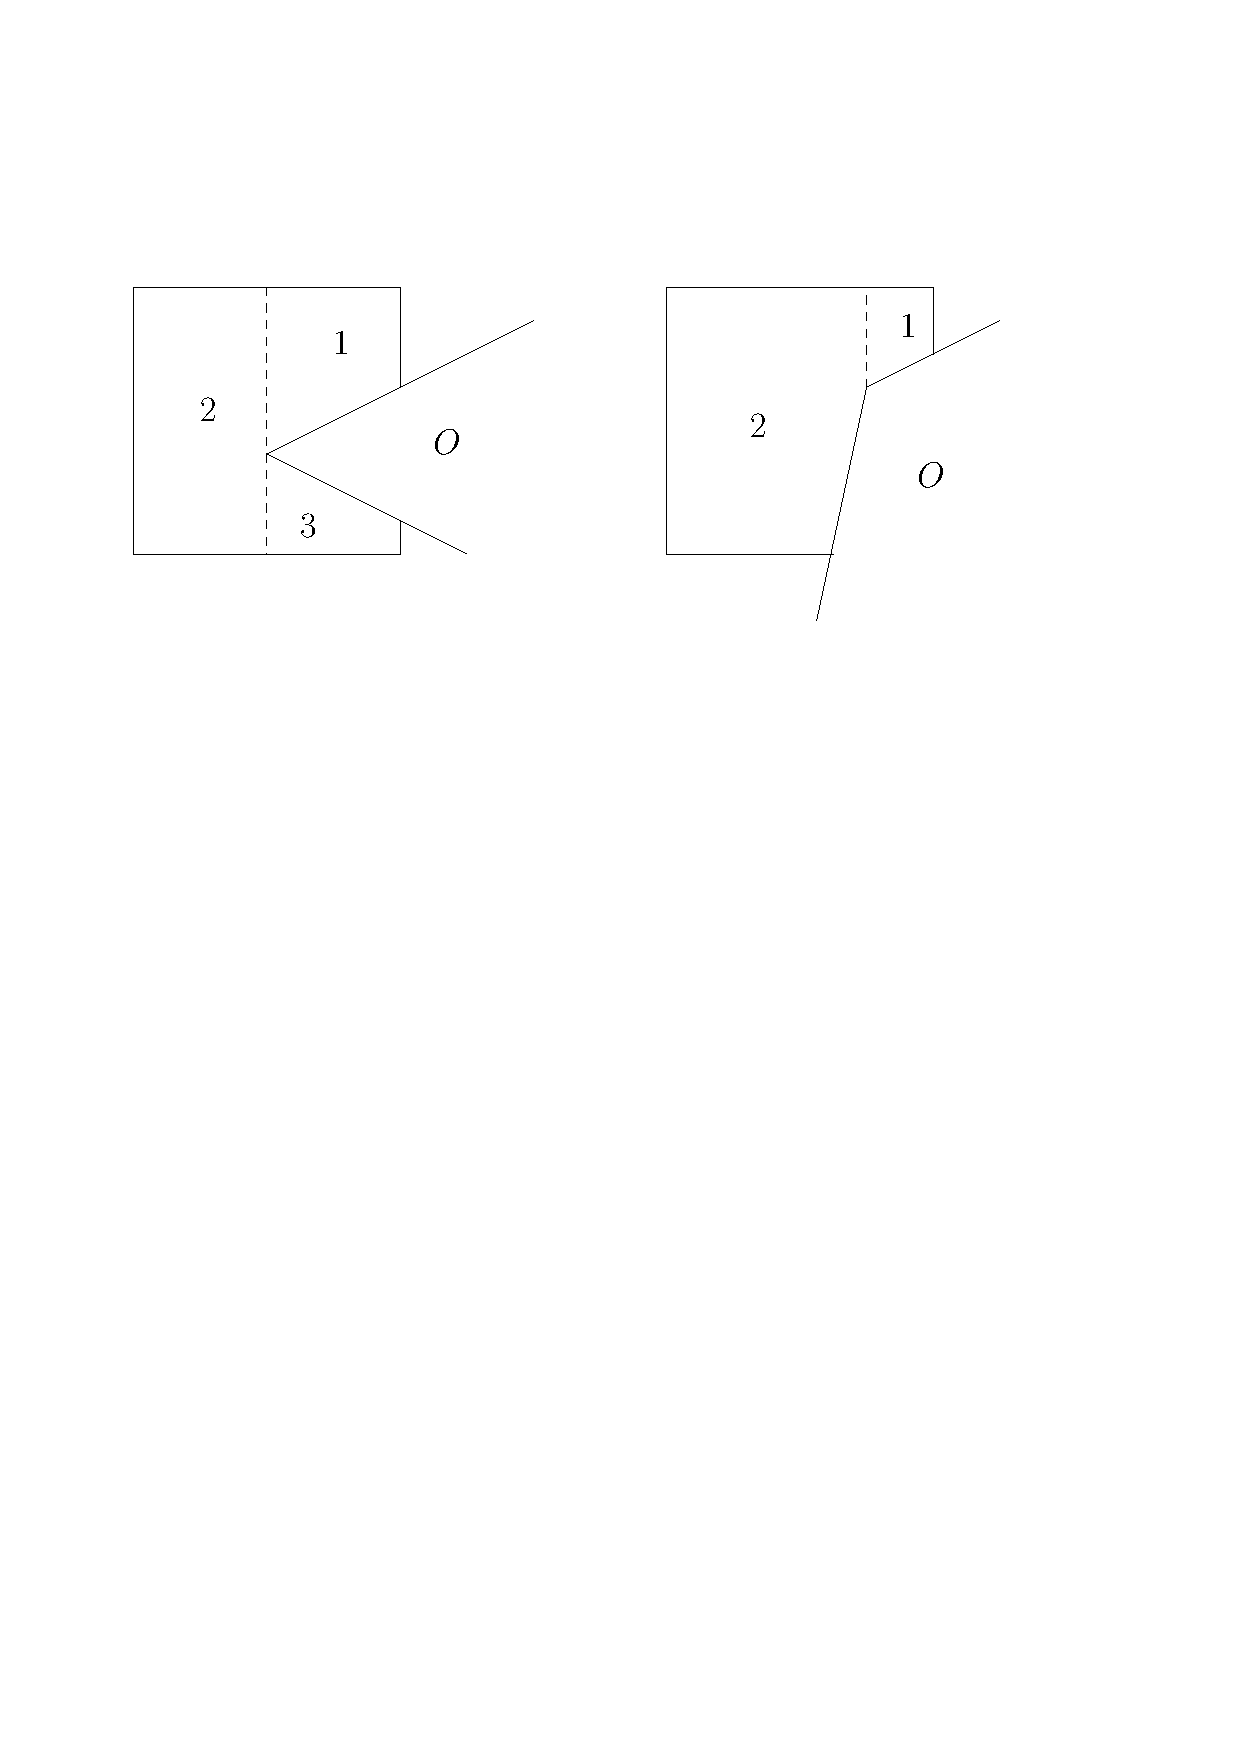
\includegraphics[width=0.8\textwidth]{figures/nonconvextoconvex.pdf}
	\caption{Left example of $v$'s added vertical edges splitting the cell into three 
    		 piece, and right example of the cell being split into two\cite{HershbergerS99}.}
	\label{fig:vinteriorinobstacle}
\end{figure}

For each such cell $c$ in $\mathcal{S}$ that contains such a $v$, let $\delta$ be the 
length of the shortest edge on the boundary of $c$ (recall that these can be subdivided). 
The newly added vertical edges are then subdivided into pieces of length at most $\delta$, 
which produces $O(1)$ vertical edge fragments. This is due to the boundary of $c$ consists 
of $O(1)$ edges, all with approximately same length and with the uniform edge property. 

We let $\mathcal{S}'$ be the result of such subdivision of cells of $\mathcal{S}$. A 
result of this is that all cells are convex excepts those derived from a square-annuli. 

Every nonconvexity in $\mathcal{S}_{overlay}$ is derived either from nonconvexity in 
$\mathcal{S}$ of $\mathcal{O}$, this is because every cell in $\mathcal{S}_{overlay}$ is 
derived from the intersection of a cell in $\mathcal{S}$ with a face of $\mathcal{O}$. 
This implies that all nonconvex cell of $\mathcal{S}_{overlay}$ are interesting cells. So 
any cell in $\mathcal{S}_{overlay}$ with an obstacles vertex inside its boundary is cut 
into convex pieces by the addition of vertical edges as was shown in Figure 
\ref{fig:vinteriorinobstacle}. So the only other nonconvex vertices in 
$\mathcal{S}_{overlay}$ are the annulus vertices. Therefore each edge fragment that is 
deleted lie on the common boundary of two uninteresting face, and its deletion therefore 
creates no new nonconvexity. 

Lets assume that a cell $c$ of $\mathcal{S}$ has $p$ edges on its boundary. Then for each 
subcell of $c$ in $\mathcal{S}'$ which contains one of $c$'s vertices will have size at most 
$2\cdot p + O(1)$, since each convex corner of $c$ may be cut off by an obstacle edge, adding 
an extra edge, and two obstacle edges may enter and exit through the same edge, leaving and 
obstacle vertex in the cell.

Adding vertical edges through each obstacle vertex splits a cell into at most three subcells, 
with at most $O(1)$ additional edges shared between them. Because each cell of $\mathcal{S}$ 
has constant complexity, then the same will be true for the interesting cells of 
$\mathcal{S}'$. From this it follows that the total complexity of the interesting cells is 
$O(n)$. Each uninteresting cell of $\mathcal{S}'$, that is those without a vertex of 
$\mathcal{S}$ or $V$, has at most eight edges. Them being four fragments from 
$\mathcal{S}$ and four from $\mathcal{O}$.

Since $\mathcal{S}'$ has $O(n)$ vertices, and each of these vertices are a vertex of an 
interesting cell, then by planarity, $\mathcal{S}'$ has $O(n)$ faces. Figure 
\ref{fig:constructingconformingsubdivision} shows a simplified example of such a construction 
of $\mathcal{S}'$. 

\begin{figure}[H]
	\centering
	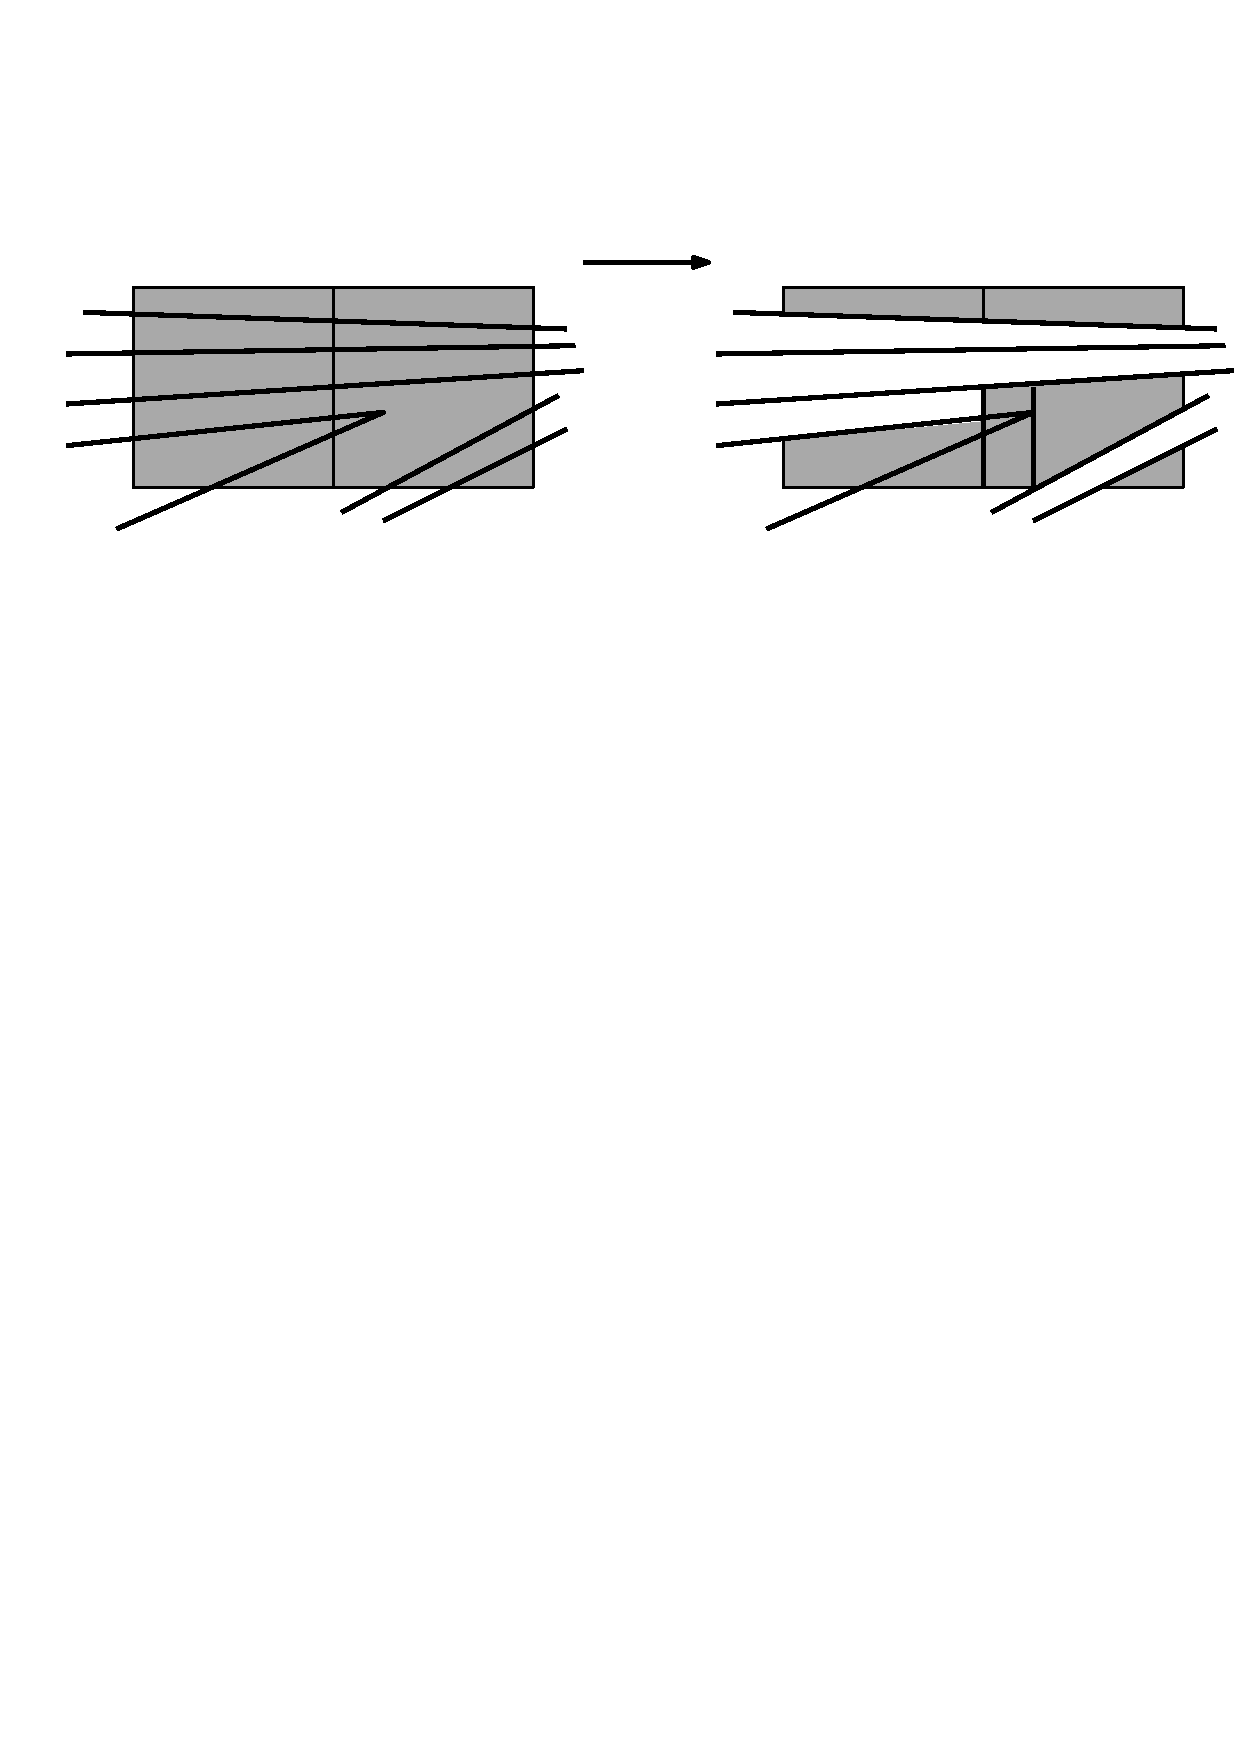
\includegraphics[width=\textwidth]{figures/constructingconformingsubdivision.pdf}
	\caption{Constructing a conforming subdivision of the free space, given a strong conforming 
    	 	 subdivision for the obstacle vertices. The shaded cells on the right are interesting 
             cells\cite{HershbergerS99}.}
	\label{fig:constructingconformingsubdivision}
\end{figure}

We will dedicate the remainder of the proof to show that the portion of $\mathcal{S}'$ outside 
all obstacles in $\mathcal{O}$ is a \textit{conforming subdivision of the free space}. So all we
to do is check the portion of $\mathcal{S}'$ outside all the obstacles in $\mathcal{O}$ behaves 
as defined by the 3 conditions from Definition \ref{def:aconformingsubdivision}

From the above it can be seen that the first condition from Definition \ref{def:aconformingsubdivision} 
is satisfied: that is each vertex of $V$ lies in its own square cell in $\mathcal{S}$. Each of 
these cells are interesting, and therefore they are either retained as they are or subdivided
in $\mathcal{S}'$. Each cell of $\mathcal{S}_{overlay}$ therefore contains at most one vertex 
of $V$ in its closure. 

To show the next condition of Definition \ref{def:aconformingsubdivision}: that is all 
transparent edges of $\mathcal{S}'$ are well-covered, which would mean they will behave as 
defined in Definition \ref{def:wellcoveringwithpara}, we consider such an edge $e'$. This 
edge $e'$ can be one of three cases: 

\begin{enumerate}
\item it may be a fragment of an edge $e\in\mathcal{S}$
\item or it may be all of $e$ s.t. $e=e'$
\item or it may be a fragment of a vertical edge added incident to an obstacle vertex.
\end{enumerate}

We will treat the first two cases as one, and for this purpose we will for the purpose of 
simplifying the notation have $\mathcal{U}=\mathcal{U}(e)$. We remind the reader 
that $\mathcal{U}(e) = \{c|c=\mathcal{C}(e)\}$ with $\mathcal{C}(e)$ being the a set of 
cells with $e$ in its interior, and $c$ being a cell. 

In the third case where $e'$ being a fragment of a vertical edge added incident to an 
obstacle vertex, $e'$ is inside a square $c$ of $\mathcal{S}$, we will define 
$\mathcal{U}=\cup_{e\in \partial c} \mathcal{U}(e)$, that is $\mathcal{U}$ is the union 
of $\mathcal{U}(e)$ over all edges of $c$'s boundary. It is worth noting that the boundary 
of $\mathcal{U}$ is covered by edge fragments from $\mathcal{S}$, and therefore also from
$\mathcal{S}_{overlay}$, but not necessarily edge fragments from $\mathcal{S}'$. Some edge 
fragments on the boundary of $\mathcal{U}$ may be erased in the construction of $\mathcal{S}'$.
That is, $\mathcal{U}$ is union of cells of $\mathcal{S}$ and therefore also of 
$\mathcal{S}_{overlay}$, but not necessarily of $\mathcal{S}'$. 

Region $\mathcal{U}$ satisfies conditions $1_{fs}$ by construction and $3_{fs}$ because 
$\mathcal{U}$ satisfies condition 3 in Definition \ref{def:wellcoveringwithpara} for 
the transparent edges of $\mathcal{S}$, and therefore for those of $\mathcal{S}_{overlay}$. 
However, it is not necessarily true that $\mathcal{U}$ is made up of a union of cells from 
$\mathcal{S}'$. This will lead to $\mathcal{U}$ being cut into a non-constant number of pieces 
by obstacle polygons. This implies we cannot use $\mathcal{U}$ directly as the well-covering 
region of $e'$ in $\mathcal{S}'$. Instead we intersect $\mathcal{U}$ with the free space, which 
will partition $\mathcal{U}$ into a connected set of components $R_1,R_2,....$. Exactly one of 
these component, e.g. $R_1$, contains $e'$. 

Next, we show that each of the $R_i$'s which are unions of cells of $\mathcal{S}_{overlay}$ is of 
constant size. This will bound the total complexity to be constant. We argue that for each cell 
$c$ in $\mathcal{S}$, a cell $c$ contains a number of $\mathcal{S}_{overlay}$ subcells, of 
which only a constant number belongs to $R_i$. "If two subcells of $c$ in $\mathcal{S}_{overlay}$
both belong to $R_i$, then the obstacle edges separating them must have endpoints either inside 
$\mathcal{U}$, or contained in one or more holes of $\mathcal{U}$ if $\mathcal{U}$ is multiply 
connected, see Figure \ref{fig:partitionedcellofu}".

\begin{figure}[H]
	\centering
	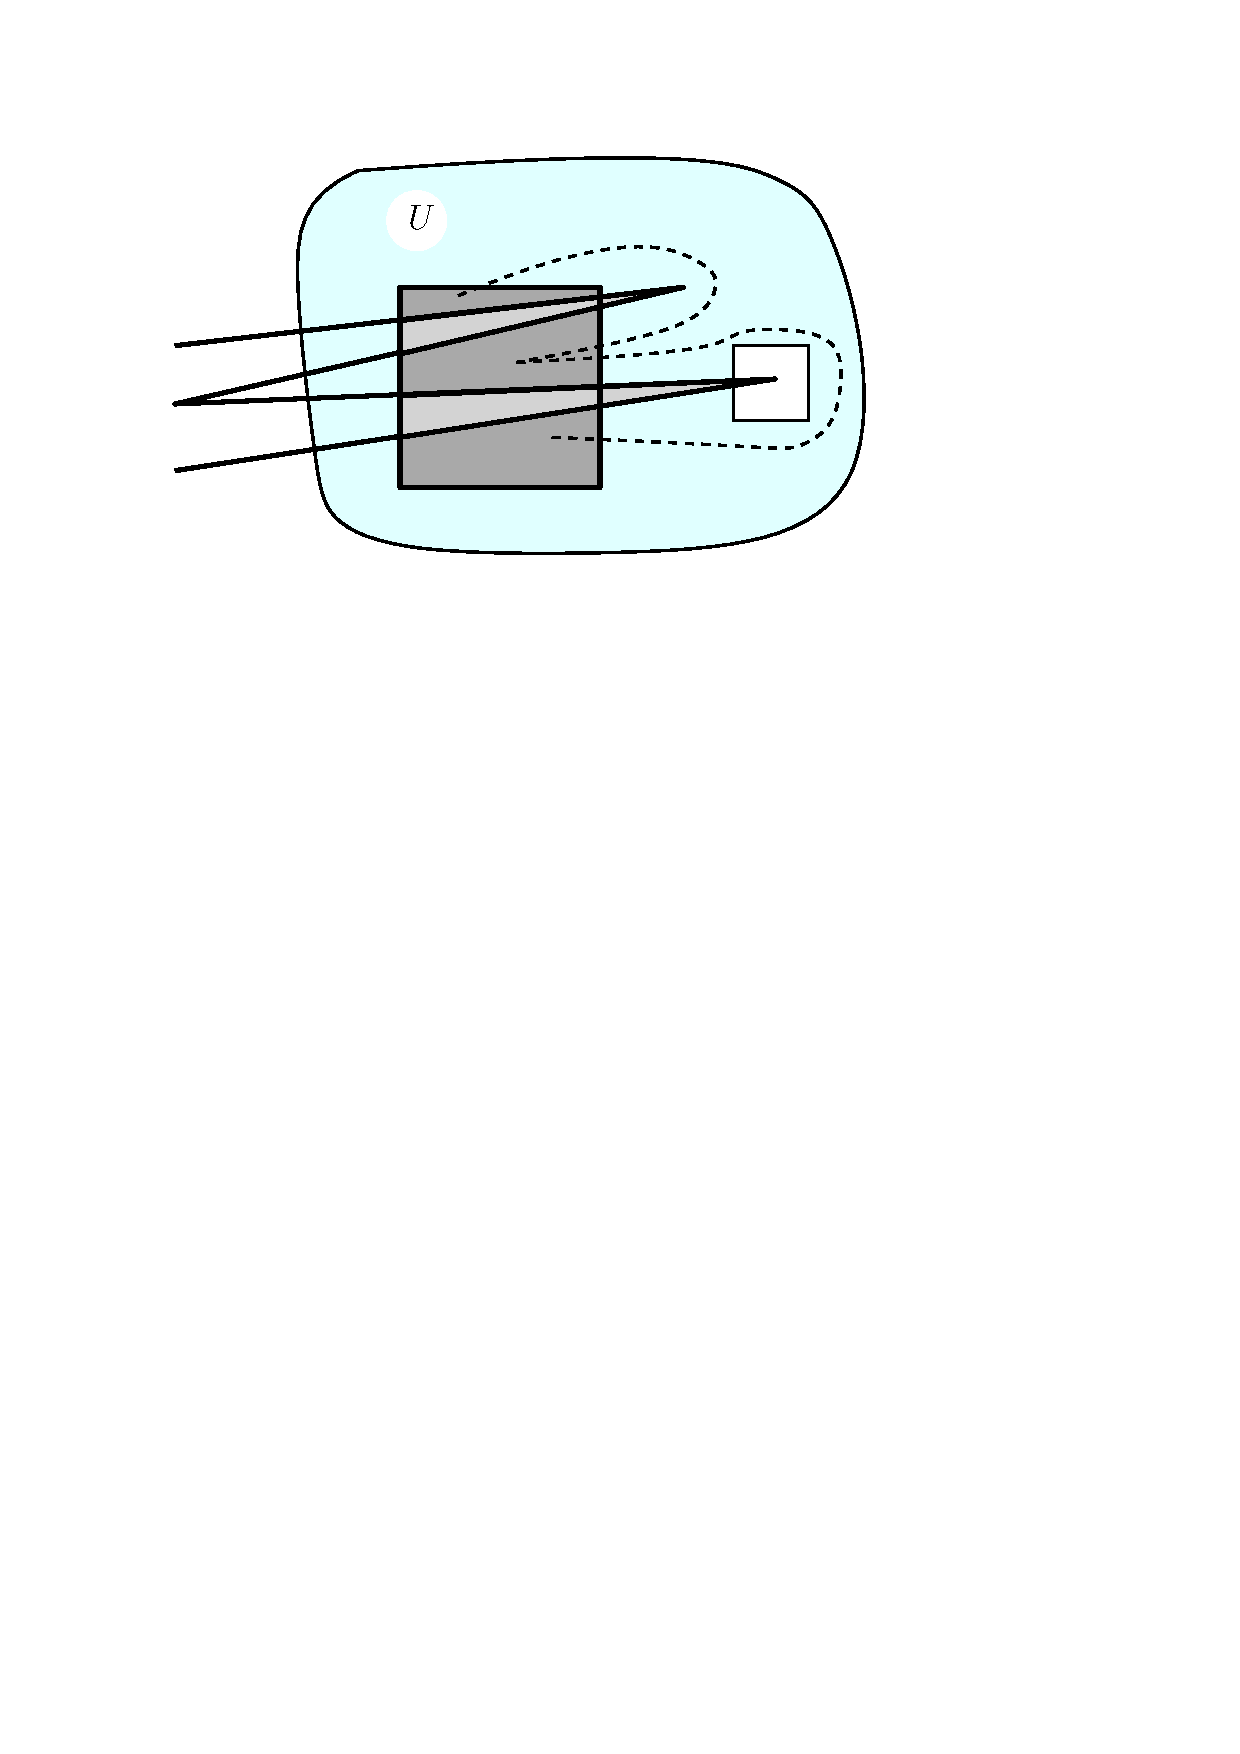
\includegraphics[width=0.8\textwidth]{figures/upartitionedintosubcells.pdf}
	\caption{A cell of $\mathcal{U}$ may be partitioned into many subcells in 
    		 $\mathcal{S}_{overlay}$, but only $O(1)$ of them belong to any one $R_i$.
             \cite{HershbergerS99}}
	\label{fig:partitionedcellofu}
\end{figure}

Were we to traverse the boundary of $R_i$, one would visit the subcells of $c$ repeatedly. 
Between each pair of different subcells of $c$, one would traverse either

\begin{enumerate}
\item A different hole of $\mathcal{U}$,
\item The outer boundary of $\mathcal{U}$, or
\item The unique obstacle vertex inside $\mathcal{U}$.
\end{enumerate}

This is due to the fact that $\mathcal{U}$ only has $O(1)$ holes, only $O(1)$ subcells 
of $c$ belong to $R_i$. 

For any given component $R_i$, let $c(R_i)$ be the cells of $\mathcal{S}_{overlay}$ in $R_i$, 
we see this mean $|c(R_i)| = O(1)$. For each cell $c\in c(R_i)$, we will have a unique cell $c'$ 
in $\mathcal{S}'$ such that $c \subseteq c'$. The cell $c$ will be strict subset of $c'$ if 
and only if some edge of $c$ was erased during the construction of $\mathcal{S}'$. 
In case that $c \subsetneq c'$, then $c'$ will be an uninteresting cell, and therefore have at 
most eight edges. This implies that both $c$ and $c'$ have constant complexity. 
If we define

$$c'(R_i)=\{c'|c'\in\mathcal{S} \text{ and } c \subseteq c' \text{ for some } c\in c(R_i)\}$$
then we have $|c'(R_i)| = O(|c(R_i)|) = O(1)$. \\

If $\mathcal{U}$ is nonconvex, it may be the case that some cell $c'$ of $\mathcal{S}'$ that 
intersects $R_i$ also intersects another component $R_j$, that is $c'(R_i)\cap c'(R_j) \neq 
\emptyset$, see Figure \ref{fig:disjointcomponentsofu}.

\begin{figure}[H]
	\centering
	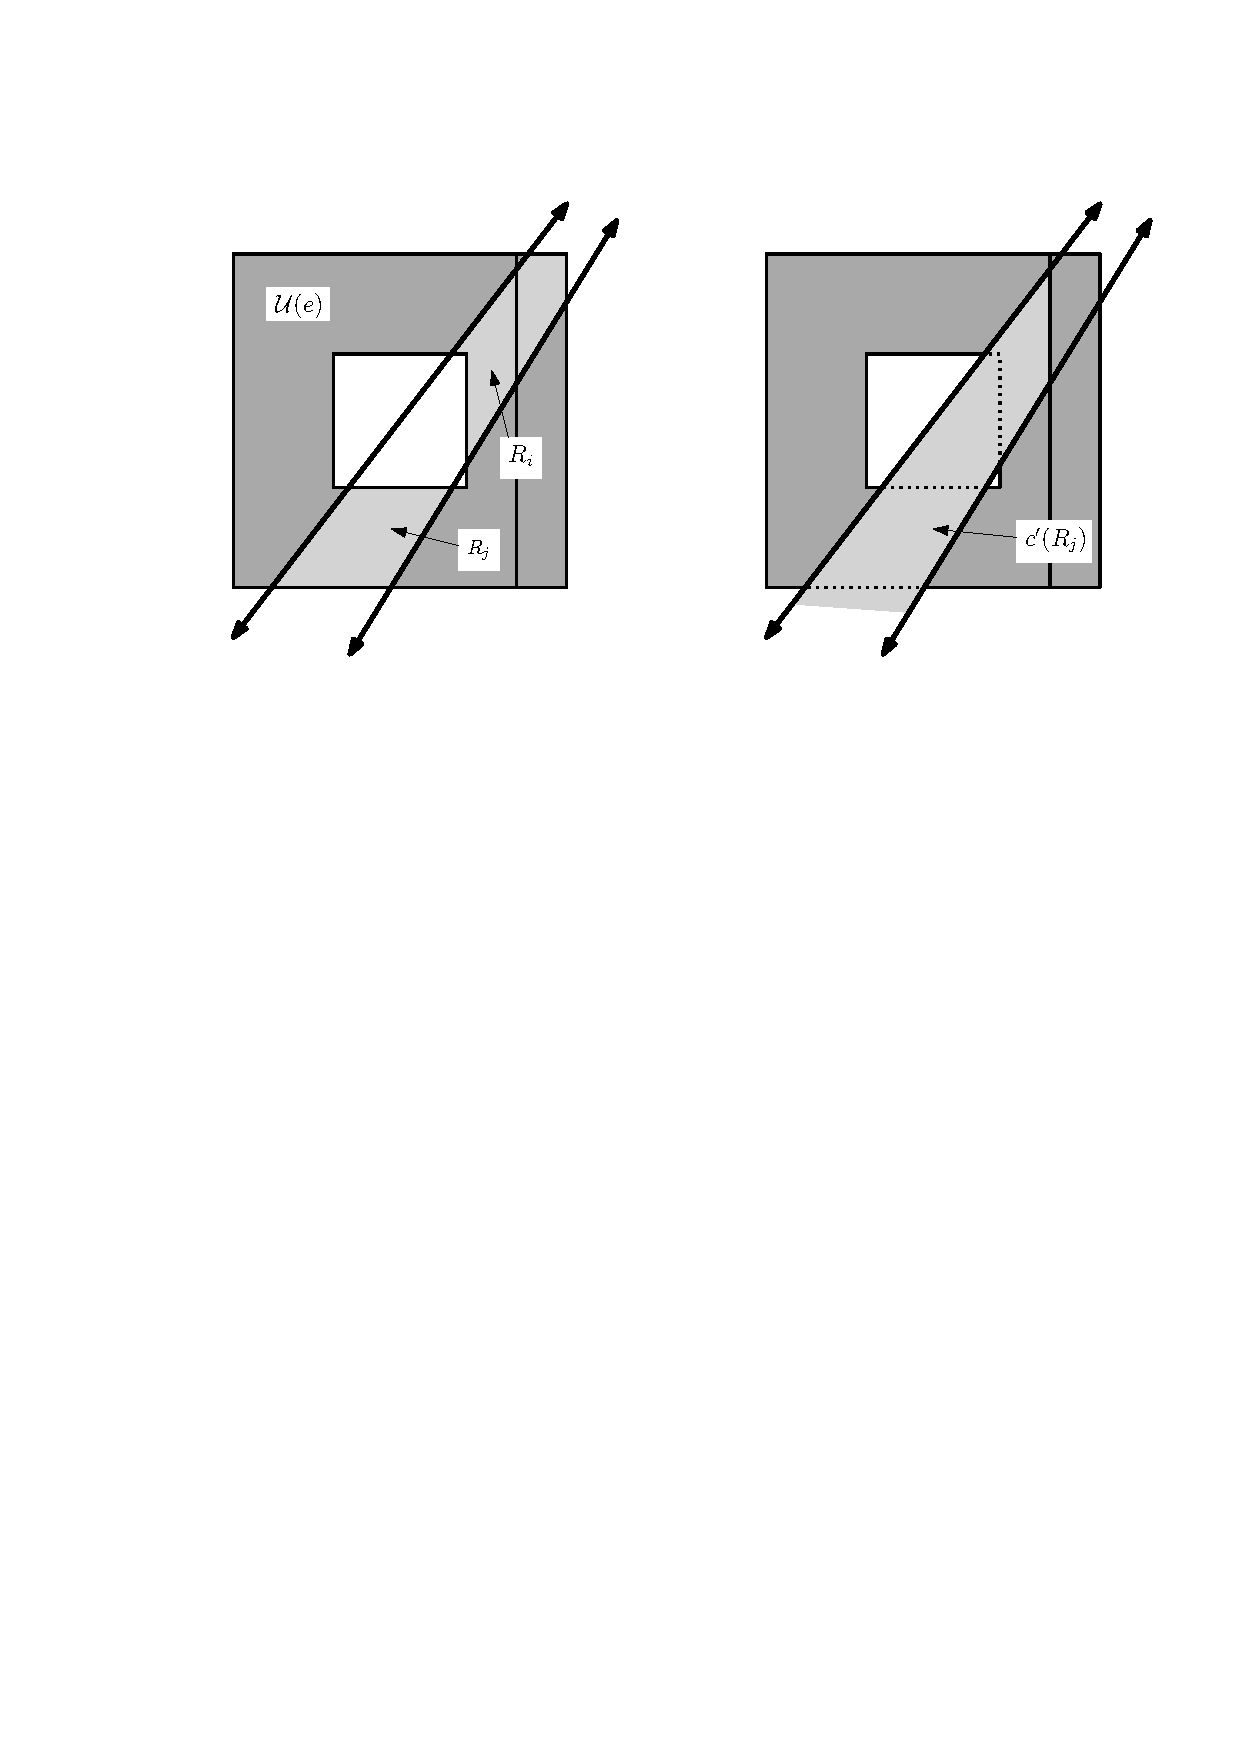
\includegraphics[width=\textwidth]{figures/disjointcomponents.pdf}
	\caption{$R_i$ and $R_j$ are disjoint components of $\mathcal{U}(e)$ in $\mathcal{S}_{overlay}$.
    		 $R_i$ is partitioned by a vertical line inside $\mathcal{U}(e)$, so $c(R_i)$ consists 
             of two cells; $c(R_j)$ is a single cell. $c'(R_j)$ intersects both $R_i$ and $R_j$, so 
             $R_i \sim R_j$. Note that $c'(r_j)$ may have transparent edges outside $\mathcal{U}(e)$. 
             \cite{HershbergerS99}}
	\label{fig:disjointcomponentsofu}
\end{figure}

Let us say that two components are connected, $R_i \sim R_j$, if and only if
$c'(R_i) \cap c'(R_j) \neq \emptyset$m and extend $\sim$ to an equivalence
relation by transitive closure.

We define $\mathcal{U}'=\mathcal{U}(e')$, the well-covering region for $e'$ in
$\mathcal{S}'$, to be the union of $c'(R_i)$ for all $R_i$ in the equivalence
class $R_1$ under the $\sim$ relation. We argue that $\mathcal{U}'$ has
constant complexity. Let $\overline{R}$ be the set of $R_i$ that contain a
vertex of $\mathcal{S}$ or $\mathcal{O}$. The set of cells
$c'(\overline{R})=\cup_{R_i\in \overline{R}}c'(R_i)$ has $O(1)$ total
complexity. Further, if $R_i\not\in\overline{R}$, then $c'(R_i)$ is a single
convex cell with $O(1)$ complexity, because all transparent edges of $c(R_i)$
inside $\mathcal{U}$ have been deleted. If such a cell $c'=c'(R_i)$ does not
intersect any component in $\overline{R}$, then the union of $c'(R_j)$ for all
$R_j\sim R_i$ is just the single cell $c'$. On the other hand, if $c'$ does
intersect some $R_j\in\overline{R}$, $c'\cup c'(R_j)$ is identical to
$c'(R_j)$. Because edge $e'$ was not deleted, $R_1\in\overline{R}$. It follows
that $\mathcal{U}'\subseteq c'(\overline{R})$, and hence $\mathcal{U}'$
satisfies condition 2 of definition 22.

The definition of $\mathcal{U}(e')$ implies that every transparent edge $f'$ on
the boundary of $\mathcal{U}(e')$ is outside or on the boundary of
$\mathcal{U}$. Edge $f'$ is a subset of some edge $f$ of $\mathcal{S}$, so the
Euclidean distance from $e'$ to $f'$ is at least $2\cdot \max(|e'|,|f'|)$. It
follows that condition $3_{fs}$ holds. Condition $1_{fs}$ holds by
construction. 

As the last thing let us establish condition 3 of definition
\ref{def:aconformingsubdivision}. A well-covering region $\mathcal{U}(e')$ in
$\mathcal{S'}$ contains no obstacle vertex that lies outside the well-covering
region $\mathcal{U} in \mathcal{S}$ from which $\mathcal{U}(e')$ is derived,
since no edges of $\mathcal{S}$ that bound vertex-containing cells are deleted.
If $e'$ is a fragment of an edge $e$ of $\mathcal{S}$ then its well-covering
region $\mathcal{U}(e')$ in $\mathcal{S}'$ contains at most one obstacle
vertex, since the same is true for $\mathcal{U}=\mathcal{U}(e)$ in
$\mathcal{S}$. If $e'$ is one of the edges added to $\mathcal{S}'$ inside a
vertex-containing square, its well-covering region $\mathcal{U}$ is the union
of $O(1)$ well-covering regions of $\mathcal{S}$. Each component region
contains the square and its vertex, and no other vertex, hence the
well-covering region of $e'$ in $\mathcal{S}'$ also satisfies condition 3 of
definition \ref{def:aconformingsubdivision}.

This complete the proof that $\mathcal{S}'$ is a conforming subdivision of the free space corresponding to the set of obstacles $\mathcal{O}$.
\end{proof}

\subsection{Lemma for efficient construction time of conforming subdivision of the free space}

The last lemma of this section shows that the conforming subdivision described above can be computed in $O(n\log n)$ time.

\begin{Lemma} (Lemma 2.3 in \cite{HershbergerS99})\\
The linear-size conforming subdivision of free space described in Lemma \ref{lemma:admitsa2conformingsubdivision} can be built in time $O(n\log n)$.
\end{Lemma}

\begin{proof}
We start with a string 2-conforming subdivision $\mathcal{S}$ of the obstacle vertices; $\mathcal{S}$ is computed in $O(n\log n)$ time, by theorem \ref{theorem:conformingsubdivision}. In $O(n\log n)$ additional time, we build a point-location data-structure for the obstacle polygons, so that given a query point $q$, we can in $O(\log n)$ times find the obstacle edge immediately to the left, right, above, or below $q$ \cite{EdelsbrunnerGS86}\cite{Kirkpatrick83}. The edges of $\mathcal{S}'$ are obstacle edges, transparent edges on the boundary of kept cell, and transparent edges incident to obstacle vertices. To identify the second kind of edges, we trace the boundary of each kept cell separately. \\

Each kept cell is contained in a single cell of $\mathcal{S}$ and has at least one vertex on its boundary, so we trace starting from each vertex. Tracing along an obstacle edge is easy, since the next transparent edge intersected is one of the $O(1)$ edges on the boundary of the current cell in $\mathcal{S}$. We use the point-location structure to trace along transparent edges: the next cell vertex is either a vertex of $\mathcal{S}$, or it is the first obstacle point hit by the ray that the current point and edge define. This tracing takes $O(n\log n)$ time altogether. The third kind of edges can be computed in $O(n)$ total time by local operations in each cell containing and obstacle vertex. To stitch the three kinds of edges into a single adjacency structure $\mathcal{S}'$, we use an $O(n \log n)$ time plane sweep algorithm \cite{CompGeo}.
\end{proof}

This complete the chapter of the conforming subdivision. 
